\chapter{串行结构的FIR滤波器设计}
\begin{introduction}
    \item \textit{通过滤波器设计工具确定滤波器系数;}
    \item \textit{Verilog编写串行结构FIR滤波器;}
    \item \textit{基于串行结构的FIR滤波器FPGA实现。}
\end{introduction}
\section{实验背景与目的}

\section{实验原理}

\section{实验使用软件/平台}
\begin{itemize}
    \item Xilinx Vivado 2024.2;
    \item eNodeX 30B软件无线电创新平台;
    \item 示波器。
    \item MATLAB \& Simulink R2024b;
  \end{itemize}
\section{实验内容}
\subsection{FIR滤波器系数确定}
打开MATLAB的\textcolor{b!50}{Filter Designer},进行如图~\ref{fig:filterdesign}~配置:
\begin{figure}
    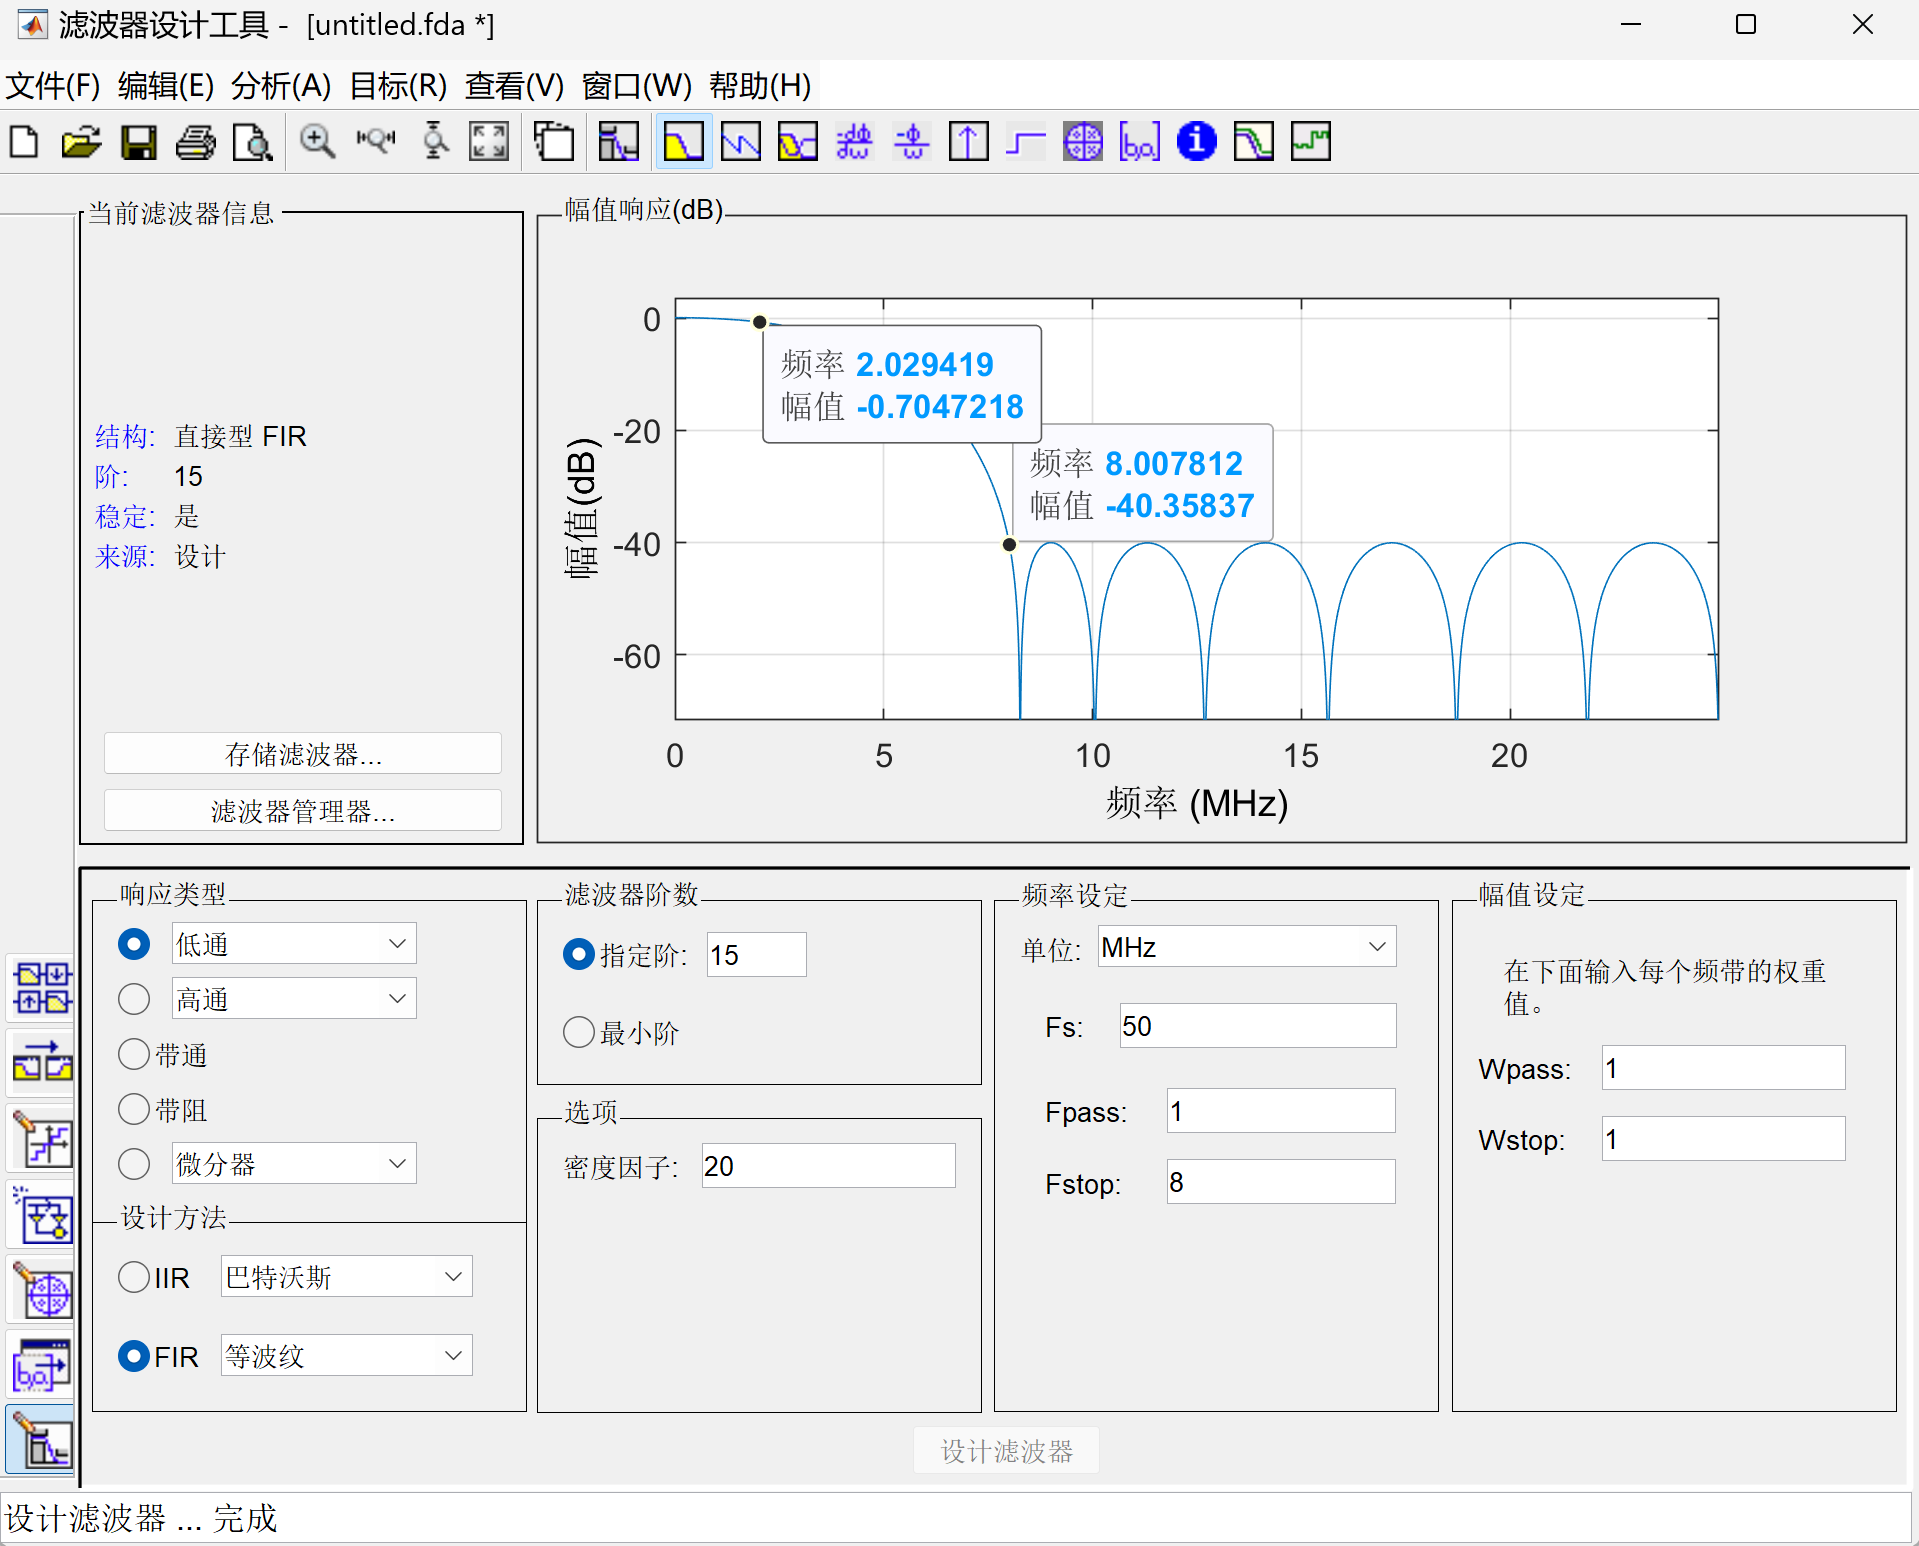
\includegraphics[width=0.45\textwidth]{figure/exp6/filter_designer.png}
    \caption{滤波器系数确定}
    \label{fig:filterdesign}
\end{figure}

在采样频率为50MHz时,该滤波器的通带边界为1MHz,阻带边界为8MHz,可以滤除
\subsection{串行结构FIR滤波器FPGA实现}
滤波器仿真结束后,连接TOP模块进行板级仿真。此次实验中,模拟输入信号由eNodeX ADC模块输入至主模块中,主模块处理好后再进行DAC输出。由于eNode X 仅有2个I/O接口,因此示波器只能显示1路信号。
\begin{lstlisting}[language=verilog,caption={TOP模块}]
`timescale 1ns / 1ps
module TOP (
    // DAC PINS
    output signed [13:0] LS_DAC2_DB,   // DA 数据2
    output               LS_DAC2_CLK,  // DA 时钟2
    output               LS_DAC2_WRT,  // DA 输出写信号,同时钟信号
    output signed [13:0] LS_DAC1_DB,   // DA 数据1
    output               LS_DAC1_CLK,  // DA 时钟1
    output               LS_DAC1_WRT,  // DA 输出写信号,同时钟信号

    output LS_DAC_MODE,

    // ADC PINS
    // input [13:0] LS_ADC2_DB, LS_ADC1_DB,     // AD 采样数据输入,目前是用的12bit ADC
    // input  LS_ADC2_OTR, LS_ADC1_OTR,         // AD 采样溢出指示(最大输入幅??2V??
    // output LS_ADC2_CLK, LS_ADC1_CLK,         // AD 采样时钟
    input [11:0] LS_ADC1_DB,
    output LS_ADC1_CLK,


    // GPIOS Ports
    // output GPIO_TH1, GPIO_TH2, GPIO_TH3, GPIO_TH4, GPIO_TH5,
    // output GPIO_TH6, GPIO_TH7, GPIO_TH8, GPIO_TH9, GPIO_TH10

    input PL_CLK_100MHz
);
  reg signed [11:0] adc1_data;

  // ADC Sampling Frequency is 6.25MHz
  always @(posedge clk_6_25M) begin
    adc1_data <= LS_ADC1_DB;
  end


  wire               clk_50M;
  wire               clk_6_25M;
  wire               clk_locked;
  wire signed [10:0] sin250k;
  wire signed [10:0] sin1M;
  wire signed [11:0] xin;
  wire signed [25:0] yout;

  clk50m inst_clk50m (
      // Clock out ports
      .clk_out_50m(clk_50M),       // output clk_out_50m
      .clk_out_625  (clk_6_25M),     // output clk_6_25M
      // Status and control signals
      .locked     (clk_locked),    // output locked
      // Clock in ports
      .clk_in1    (PL_CLK_100MHz)  // input clk_in1
  );

  ila_0 inst_ila (
      .clk(clk_50M),
      .probe0(adc1_data),
      .probe1(yout[25:12]),
      .probe2(xin)
  );



  fir_serial sim (
      .rst (!clk_locked),
      .clk (clk_50M),
      .Xin (adc1_data),
      .Yout(yout)
  );

  SIN_1M sin_1M (
      .aclk                (clk_50M),  // input wire aclk
      .s_axis_config_tvalid(1'b1),     // input wire s_axis_config_tvalid
      .s_axis_config_tdata (16'H51E),  // input wire [11 : 0] s_axis_config_tdata
      .m_axis_data_tvalid  (),         // output wire m_axis_data_tvalid
      .m_axis_data_tdata   (sin1M)     // output wire [11 : 0] m_axis_data_tdata
  );
  SIN_1M sin_0_25M (
      .aclk                (clk_50M),  // input wire aclk
      .s_axis_config_tvalid(1'b1),     // input wire s_axis_config_tvalid
      .s_axis_config_tdata (16'H147),  // input wire [15 : 0] s_axis_config_tdata
      .m_axis_data_tvalid  (),         // output wire m_axis_data_tvalid
      .m_axis_data_tdata   (sin250k)   // output wire [15 : 0] m_axis_data_tdata
  );

  // 计算输入信号
  assign xin = sin1M + sin250k;
  // DAC OUTPUT
  assign LS_DAC_MODE = 1'b1;
  assign LS_DAC1_DB = {{2{xin[11]}}, xin} + 14'h2000;  // to unsigned
  assign LS_DAC1_CLK = !clk_50M;
  assign LS_DAC1_WRT = LS_DAC1_CLK;
  assign LS_DAC2_DB = yout[25:12] + 14'h2000;  // to unsigned
  assign LS_DAC2_CLK = clk_50M;
  assign LS_DAC2_WRT = LS_DAC2_CLK;

  assign LS_ADC1_CLK = clk_6_25M;
endmodule

\end{lstlisting}
\subsection{FPGA资源消耗分析}
首先将该并行滤波器\textbf{设置为顶层模块},并\textbf{禁用}TOP模块。然后通过命令行或\texttt{Add Timing Constraints}绑定时钟管脚\texttt{clk}至50MHz时钟。此时Vivado便可以不通过实际开发板完成资源消耗分析。

完成Implementation后,打开Report Utilization便可看到该模块的资源消耗情况如图~\ref{fig:exp6:util}。
\begin{figure}[htbp]
  \centering
  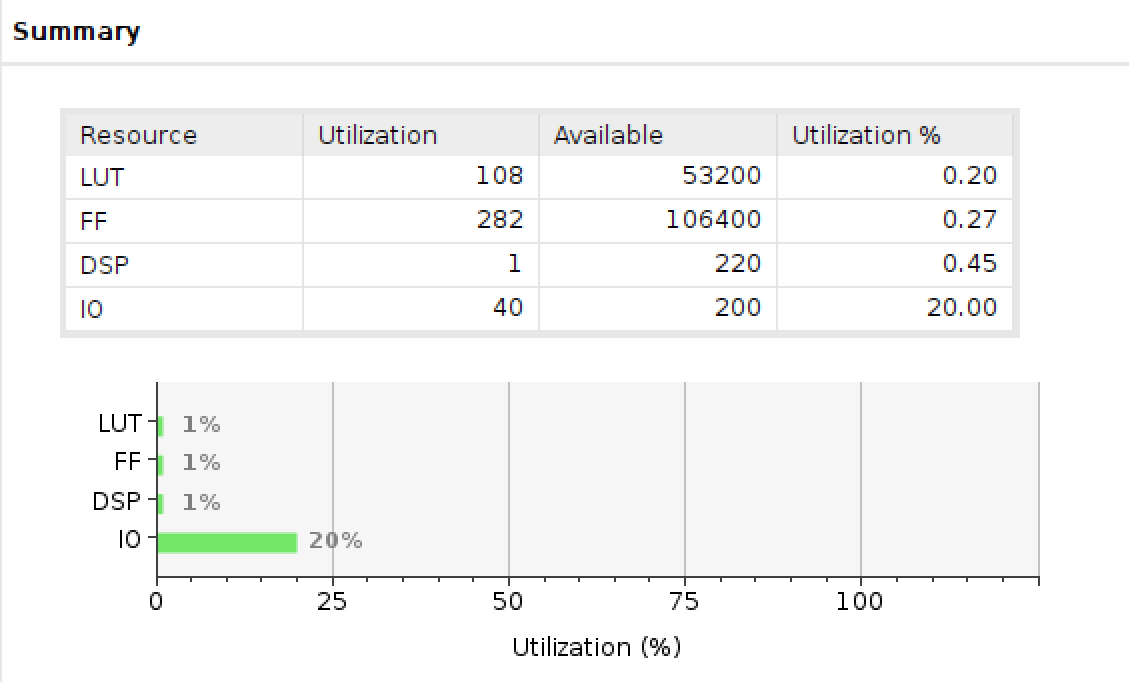
\includegraphics[width=0.55\textwidth]{figure/exp6/util_summary.png}
  \caption{串行结构FIR滤波器资源消耗分析}
  \label{fig:exp6:util}
\end{figure}

该设计的 LUT 和 FF 的资源消耗都很低,但IO资源的消耗较高(20\%),这是因为输入输出的位宽较大,属于刚性需求。并且可以看出,在Implementation的过程中,布线器对资源进行了优化。总消耗资源并不等于每个子模块的资源消耗之和。

\subsection{时序检查报告}

图~\ref{fig:exp6:timing}~展示了FPGA设计的时序总结,包括Setup、Hold和Pulse Width三个方面的时序检查结果。

\begin{figure}[htbp]
  \centering
  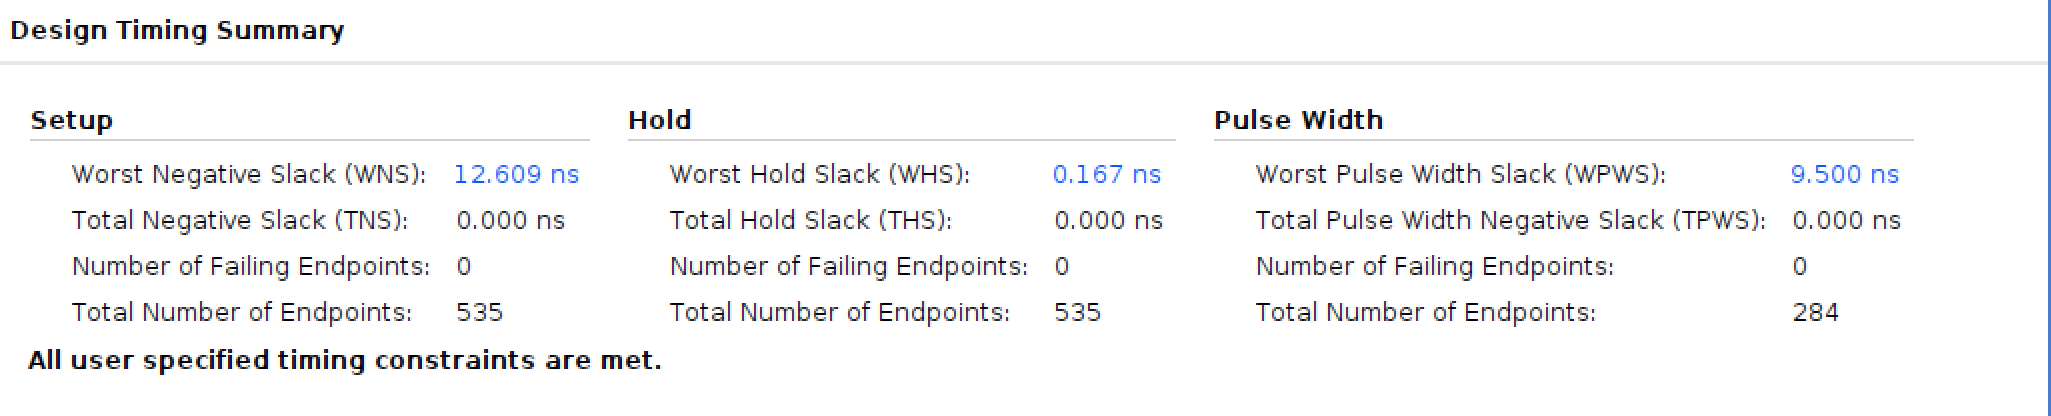
\includegraphics[width=0.75\textwidth]{figure/exp6/timing_summary.png}
  \caption{模块时序检查报告}
  \label{fig:exp6:timing}
\end{figure}


\textbf{Setup:}  
\begin{itemize}
  \item Worst Negative Slack (WNS): 12.635 ns。表示最差的负时序余量,值为12.635纳秒,说明在时序上存在一定的余量,设计没有违反时序约束。  
\item Total Negative Slack (TNS): 0.00 ns。表示总的负时序余量为零,说明所有时序约束都被满足。  
\item Number of Failing Endpoints: 0。表示没有时序失败的端点,所有的时序约束都符合要求。  
\item Total Number of Endpoints: 535。表示在设计中,共有535个时序端点。
\end{itemize}


\textbf{Hold:}  
\begin{itemize}
\item Worst Hold Slack (WHS): 0.167 ns。表示最差的保持时序余量,值为0.167纳秒,表明该设计在保持时序方面没有违反约束。  
\item Total Hold Slack (THS): 0.00 ns。表示总的保持时序余量为零,表明所有保持时序约束都被满足。  
\item Number of Failing Endpoints: 0。表示没有违反保持时序约束的端点。  
\item Total Number of Endpoints: 535。表示共有535个端点。
\end{itemize}

\textbf{Pulse Width:}  
\begin{itemize}
  \item Worst Pulse Width Slack (WPWS): 9.500 ns。表示最差的脉冲宽度时序余量,值为9.500纳秒,说明设计在脉冲宽度方面有足够的时序余量。  
  \item Total Pulse Width Negative Slack (TPWS): 0.00 ns。表示总的脉冲宽度负时序余量为零,表明所有脉冲宽度时序约束都得到满足。  
  \item Number of Failing Endpoints: 0。表示没有违反脉冲宽度时序约束的端点。  
\item Total Number of Endpoints: 284。表示共有284个端点。
\end{itemize}


\textbf{总结:}  
所有用户指定的时序约束都已满足,设计没有违反时序约束,时序余量充足,表明该设计的时序性能良好,符合要求。

\section{思考与讨论}
\subsection{半串行结构FIR滤波器}
为了提高工作频率,采用两个乘法器和两个加法器完成FIR滤波器的设计。此时设计的滤波器代码为:
\begin{lstlisting}[language=verilog]
module FIR_HALF_SERIAL (
    input rst,  // Async reset on posedge            
    input clk,  // system clock                    
    input signed [11:0] Xin,  // 12-bit input
    output reg signed [25:0] Yout  // adder output
);
  reg signed [11:0] coe_a, coe_b;  // coefficients for two separate operations
  wire signed [12:0] add_s1, add_s2;  // intermediate adders' results

  reg [2:0] count = 3'd0;  
  always @(posedge clk or posedge rst) begin
    if (rst) count <= 3'd0;
    else begin
      if (count == 3'd4) begin
        count <= 0;
      end else begin
        count <= count + 1;
      end
    end
  end

  reg [11:0] Xin_Reg[15:0];  // Data shift register
  // reg [3:0] i, j; 

  // Store data into the shift register
  always @(posedge clk or posedge rst) begin
    if (rst) begin
      // Initialize register values to 0
      Xin_Reg[0]  <= 12'd0;
      Xin_Reg[1]  <= 12'd0;
      Xin_Reg[2]  <= 12'd0;
      Xin_Reg[3]  <= 12'd0;
      Xin_Reg[4]  <= 12'd0;
      Xin_Reg[5]  <= 12'd0;
      Xin_Reg[6]  <= 12'd0;
      Xin_Reg[7]  <= 12'd0;
      Xin_Reg[8]  <= 12'd0;
      Xin_Reg[9]  <= 12'd0;
      Xin_Reg[10] <= 12'd0;
      Xin_Reg[11] <= 12'd0;
      Xin_Reg[12] <= 12'd0;
      Xin_Reg[13] <= 12'd0;
      Xin_Reg[14] <= 12'd0;
      Xin_Reg[15] <= 12'd0;
    end else begin
      if (count == 3'd4) begin
        // Shift data in the register every time count == 4
        Xin_Reg[15] <= Xin_Reg[14];
        Xin_Reg[14] <= Xin_Reg[13];
        Xin_Reg[13] <= Xin_Reg[12];
        Xin_Reg[12] <= Xin_Reg[11];
        Xin_Reg[11] <= Xin_Reg[10];
        Xin_Reg[10] <= Xin_Reg[9];
        Xin_Reg[9]  <= Xin_Reg[8];
        Xin_Reg[8]  <= Xin_Reg[7];
        Xin_Reg[7]  <= Xin_Reg[6];
        Xin_Reg[6]  <= Xin_Reg[5];
        Xin_Reg[5]  <= Xin_Reg[4];
        Xin_Reg[4]  <= Xin_Reg[3];
        Xin_Reg[3]  <= Xin_Reg[2];
        Xin_Reg[2]  <= Xin_Reg[1];
        Xin_Reg[1]  <= Xin_Reg[0];
        Xin_Reg[0]  <= Xin;
      end
    end
  end


  reg signed [11:0] add_a1, add_b1, add_a2, add_b2;

  always @(posedge clk or posedge rst) begin
    if (rst) begin
      add_a1 <= 12'd0;
      add_b1 <= 12'd0;
      add_a2 <= 12'd0;
      add_b2 <= 12'd0;
      coe_a  <= 12'd0;
      coe_b  <= 12'd0;
    end else begin
      // Select different coefficients for two separate operations based on the count value
      case (count)
        3'd0: begin
          add_a1 <= Xin_Reg[0];
          add_b1 <= Xin_Reg[15];
          coe_a  <= -12'd116;  // c0
          add_a2 <= Xin_Reg[1];
          add_b2 <= Xin_Reg[14];
          coe_b  <= -12'd111;  // c1
        end
        3'd1: begin
          add_a1 <= Xin_Reg[2];
          add_b1 <= Xin_Reg[13];
          coe_a  <= -12'd22;  // c2
          add_a2 <= Xin_Reg[3];
          add_b2 <= Xin_Reg[12];
          coe_b  <= 12'd243;  // c3
        end
        3'd2: begin
          add_a1 <= Xin_Reg[4];
          add_b1 <= Xin_Reg[11];
          coe_a  <= 12'd692;  // c4
          add_a2 <= Xin_Reg[5];
          add_b2 <= Xin_Reg[10];
          coe_b  <= 12'd1239;  // c5
        end
        3'd3: begin
          add_a1 <= Xin_Reg[6];
          add_b1 <= Xin_Reg[9];
          coe_a  <= 12'd1743;  // c6
          add_a2 <= Xin_Reg[7];
          add_b2 <= Xin_Reg[8];
          coe_b  <= 12'd2047;  // c7
        end
        default: begin
          add_a1 <= 12'd0;
          add_b1 <= 12'd0;
          coe_a  <= 12'd0;
          add_a2 <= 12'd0;
          add_b2 <= 12'd0;
          coe_b  <= 12'd0;
        end
      endcase
    end
  end

  // Add two separate sums
  ADDER u2_1 (
      .A(add_a1),
      .B(add_b1),
      .S(add_s1)
  );

  ADDER u2_2 (
      .A(add_a2),
      .B(add_b2),
      .S(add_s2)
  );

  wire signed [24:0] Mout1, Mout2;  // Output from two multipliers

  // Two separate multipliers, one for each sum
  MULT u1_1 (
      .CLK(clk),
      .A  (add_s1),
      .B  (coe_a),
      .P  (Mout1)
  );

  MULT u1_2 (
      .CLK(clk),
      .A  (add_s2),
      .B  (coe_b),
      .P  (Mout2)
  );

  reg signed [25:0] sum;

  always @(posedge clk or posedge rst) begin
    if (rst) begin
      sum  <= 26'd0;
      Yout <= 26'd0;
    end else begin
      // Accumulate the results from both multipliers
      sum <= sum + Mout1 + Mout2;
      if (count == 3'd2) begin  // Reset accumulator on count == 2
        Yout <= sum;  // Output the filtered result
        sum  <= 26'd0;  // Clear sum
      end
    end
  end

endmodule
\end{lstlisting}

相较原有代码,新的滤波器频率提高了一倍,然而仿真结果(图~\ref{fig:half_serial}~)显示其低通滤波效果很差。这是因为随着滤波器设计(尤其是采样频率)的改变,滤波器系数需要重新设计。滤波器系数的取值详见MATLAB实验部分,此处不再展开。
\begin{figure}[htbp]
    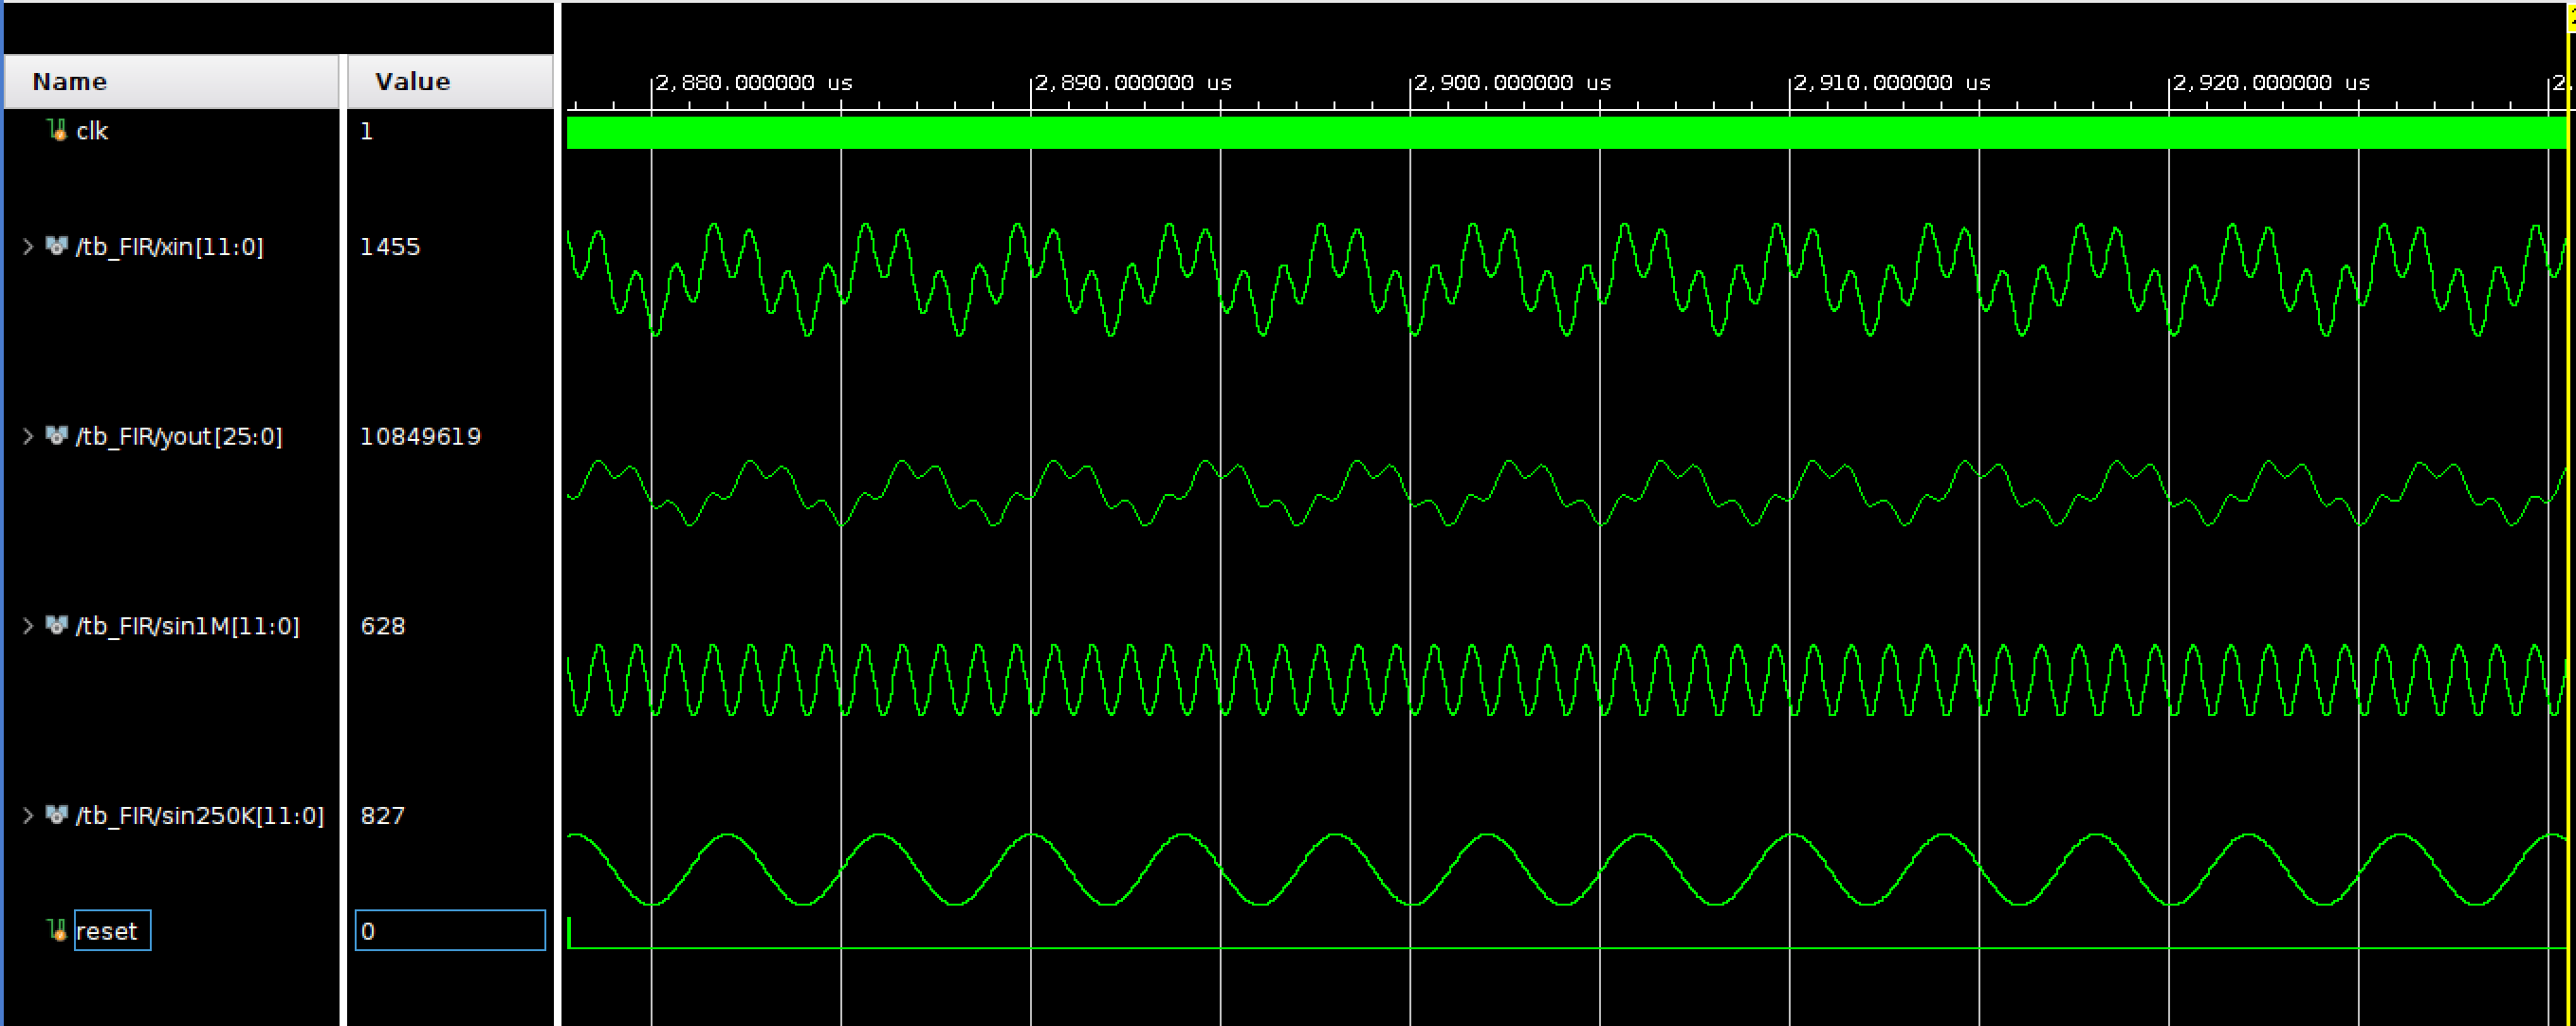
\includegraphics[width=0.95\textwidth]{figure/exp6/waveform_2adders.png}
    \caption{半串行结构的FIR滤波器滤波效果仿真}
    \label{fig:half_serial}
\end{figure}
